\chapter{Background and related Work}
\label{ch:background}
Background Intro

The Background chapter helps the reader understand the relevance of your research, the challenges you are tackling, and why your research is needed in the first place.
Provides the context, motivation, and justification for your research. It focuses on what the problem is, why it is important, and where your research fits into the broader landscape.

\section{Background}
\label{sec:background:background}
simmilar to motivation, what is the present state of volunteer computing? what is my addition?

Why do we choose the Web (especially Browser) environment and what is the current state of the browser?

\section{Theory}
\label{sec:background:theory}
This following section displays the mathematical and theoretical background of a distributed computing network. The objective is to identify the constraints that must be satisfied to ensure that the use of a distributed computing network offers advantages over regular local computing on a single device.

The primary constraint is that the program code, which is distributed across multiple devices, must be capable of parallel execution. This allows all participating devices to  each compute a portion of the overall workload simultaneously. In this context, a parallelizable problem, as defined in this thesis, is characterized by the following properties:
\begin{itemize}
    \item The problem can be divided into multiple tasks.
    \item Each task executes the same program code.
    \item Each task can receive specific input parameters to process a distinct part of the problem.
    \item Each task operates independently, with no need for communication between tasks.
\end{itemize}
To calculate the execution time of a parallelizable problem, the problem is divided into \emph{T} equally sized tasks. It is assumed that, on average, each task requires a computing time of $t_{C}$ when executed on a single device. Consequently, the total computation time for a parallelizable problem on a single device is expressed as:
\begin{equation}
T \cdot t_{C}
\label{equ:single}
\end{equation}
When the tasks \emph{T} are executed in parallel on \emph{N} nodes, the total computation time is reduced proportionally by distributing the workload. This is implemented through the fraction of \emph{T} and \emph{N}. Since \emph{T}, \emph{N} and the result of their division need to be natural numbers ($\mathbb{N}$), the gaussian ceiling function is applied. The ceiling function values any remainder as a additional value when dividing tasks among nodes and therefore always returns a value in range of $\mathbb{N}$. Hence, the fraction is given by: 
\begin{equation}
\bigg\lceil\frac{T}{N}\bigg\rceil
\label{equ:frac}
\end{equation}
When a problem is distributed across \emph{N} nodes over a wireless connection, the network latency must be taken into account in the computation. The latency, denoted as $t_{L}$, consists of the time required to send input arguments to a single device and the time needed to receive the result from a single task. It is assumed that the program code necessary to execute a task is loaded on all devices in advance, and therefore, the initial overhead of this process is excluded from the calculation. Additionally, it is assumed that the computation time, $t_{C}$, is equally long across all \emph{N} nodes. Thus, the total execution time for a parallelizable problem distributed across \emph{N} nodes can be expressed as: 
\begin{equation}
\bigg\lceil\frac{T}{N}\bigg\rceil \cdot (t_{C} + t_{L})
\label{equ:multiple}
\end{equation}
The objective is to reduce the total computation time of a problem by distributing the workload across multiple nodes in parallel. This means that the execution time on a single device, as described by \eqref{equ:single}, must be longer than the execution time on multiple devices, as described by \eqref{equ:multiple}. This leads to following inequality expression:
\begin{equation}
T \cdot t_{C} > \bigg\lceil\frac{T}{N}\bigg\rceil \cdot (t_{C} + t_{L})
\label{equ:compare}
\end{equation}
In order to transform this inequality, the term needs to be simplified by substituting the gaussian bracket. The fraction \eqref{equ:frac} can be replaced by an overestimate, without altering the logical validity of the inequality:
\begin{equation}
\bigg\lceil\frac{T}{N}\bigg\rceil < \frac{T}{N} + 1
\label{equ:frac2}
\end{equation}
Substituting this overestimate into the inequality allows for the following transformation:
\begin{alignat}{4}
 T \cdot t_{C} &> \bigg(\frac{T}{N} + 1\bigg) \cdot (t_{C} + t_{L}) \nonumber \\
 T \cdot t_{C} &> \bigg(\frac{T + N}{N}\bigg) \cdot (t_{C} + t_{L}) \nonumber \\
 \frac{T \cdot N \cdot t_{C}}{T + N} &> t_{C} + t_{L} \nonumber \\
 \frac{T \cdot N \cdot t_{C}}{T + N} - t_{C} &> t_{L} \nonumber \\
 t_{C} \cdot \bigg(\frac{T \cdot N}{T + N} - 1\bigg) &> t_{L}
 \label{equ:transformation}
\end{alignat}
The last expression through the transformation in \eqref{equ:transformation} results in the constrain, that distributing a parallelizable problem across multiple nodes is only beneficial if the latency $t_{L}$ is shorter than the computation time of a single task multiplied by the factor $(\frac{T \cdot N}{T + N} - 1)$.

Additionally the expression \eqref{equ:frac} can be used to determine the optimal amount of nodes \emph{N} for a problem divided in \emph{T} equally sized tasks. This expression reaches its minimum when \emph{N} equals \emph{T}. This outcome is intuitive, as in this ideal scenario each Node is rersponsible for a single task and therefore all tasks \emph{T} are executed simultaneously. Furthermore can be concluded from \eqref{equ:frac} that the amount of nodes should ideally be a divisor of \emph{T} to ensure a efficient utilization of all nodes. However, in practice, it should be considered to include additional backup devices in the network to account for potential failures or disruptions.

\subsection{Theoretical Case}
To illustrate the performance gain achieved by a distributed computing network, both expressions \eqref{equ:single} and \eqref{equ:multiple} are plotted in figure \ref{fig:background:theoryplot}. To calculate these graphs, an Internet latency of 32 ms \cite{backend:latency} was assumed. This value is the \ac{IQI} estimated round trip time within Europe \cite{backend:latency}. The average computation time $t_{C}$ for a single task was assumed to be 614 ms, based on the measured average run time of the example code in \ref{app:code:mandelbrot1} on the system specified in \ref{app:system:mymachine}.

An initial setup offset is additionally considered to establish the distributed computing network. In this process, each node must download all necessary files in advance to be able to execute the workload. Since this setup occurs in parallel across all nodes, the offset matches the time required for the setup of a single node. This offset value is calculated using the \ac{IQI} estimated download speed in Europe of 29 Mbps \cite{backend:latency}. The size of the compiled WebAssembly binary file from the source code in \ref{app:code:mandelbrot2} is 1096 Kb (137 KB), and the coresponding generated Gluecode JavaScript file is 129 Kb (24 KB), resulting in a total file size of 1225 Kb. The time required to download both files to a single node can be estimated using the following expression:
\begin{equation}
 Offset = Latency + (\frac{Filesize}{Bandwith} \cdot 1000) 
 \label{equ:offset}
\end{equation}
Since the latency is given in milliseconds, while the bandwidth is provided in megabits per second, the unit of the result from expression \ref{equ:offset} is converted to milliseconds by multiplying the download time by 1000. Using this calculation, the additional offset required to set up the platform in this theoretical case is estimated to be at least 75 ms. The source code to generate both graphs of figure \ref{fig:background:theoryplot} can be found in section \ref{app:code:theoryplots}.

\begin{figure}[bth]
  \myfloatalign
  \subfloat[Variable amount of nodes N]{
     \label{fig:background:theoryA}
     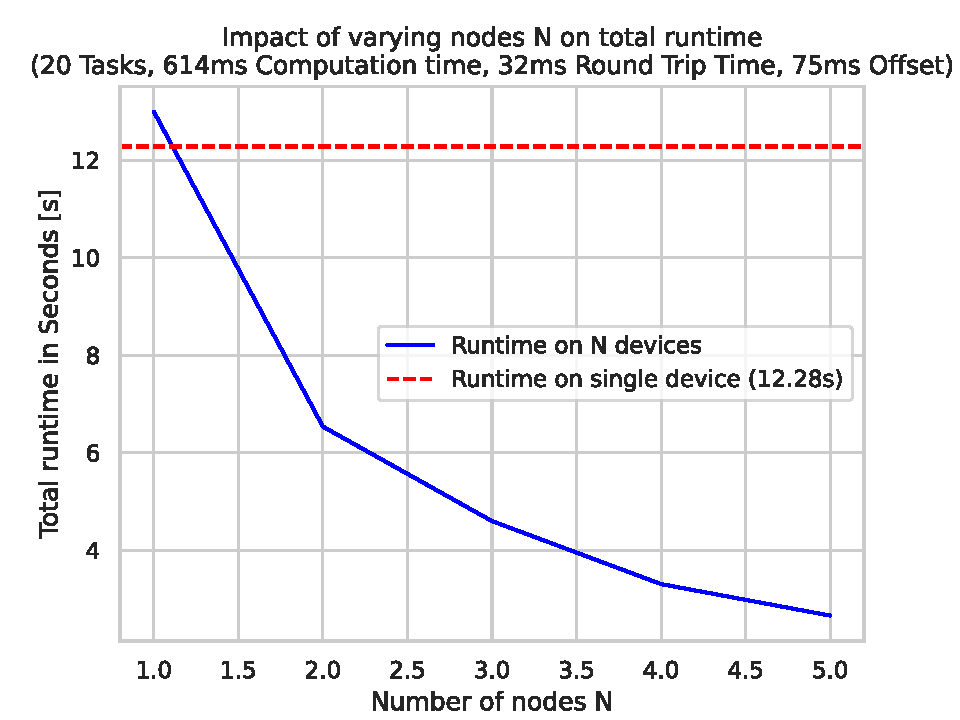
\includegraphics[width=.45\linewidth]{gfx/figures/Theory_A.pdf}
   }
   \subfloat[Variable amount of tasks T]{
     \label{fig:background:theoryB}
     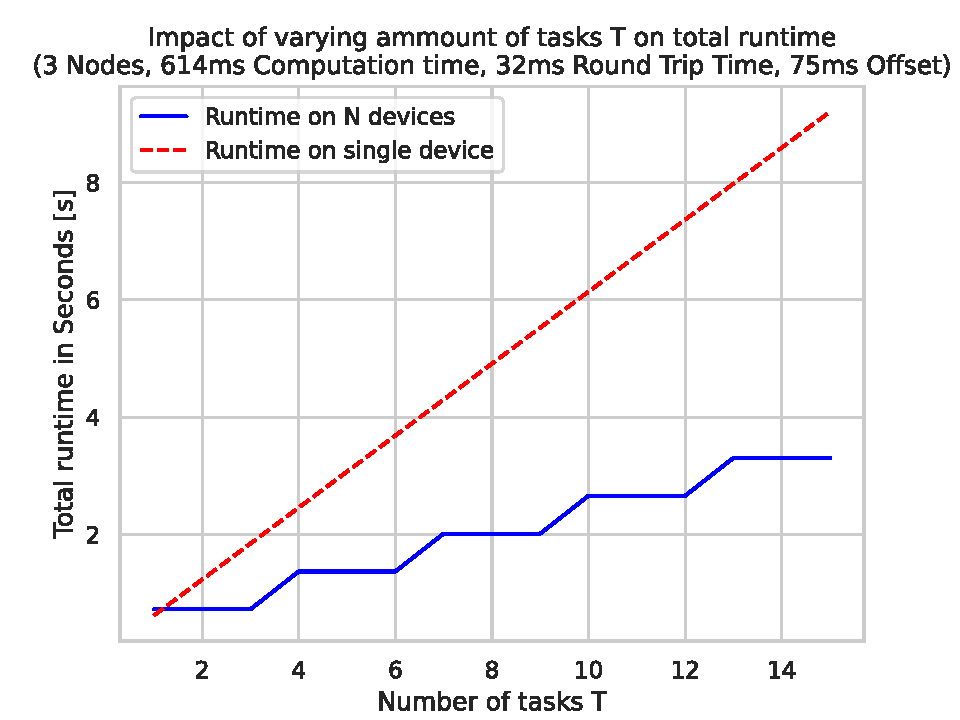
\includegraphics[width=.45\linewidth]{gfx/figures/Theory_B.pdf}
   }
   \caption{Visualizing the Total Computation Time for an Estimated Example Case}
   \label{fig:background:theoryplot}
\end{figure}

TODO: Explain graphs here

\section{Related Work}
\label{sec:background:related_work}
This Sections introduces related Works in this field topic from the past and present
\subsection{SETI@home}
\label{subsec:background:related_work:seti}
Informations about SETI
\subsection{BOINC}
\label{subsec:background:related_work:boinc}
Informations about BOINC
\subsection{XtremWeb}
\label{subsec:background:related_work:xtremweb}
Informations about XtremWeb
\subsection{EGEE}
\label{subsec:background:related_work:egee}
Informations about EGEE
\subsection{Island Paper Wasm}
\label{subsec:background:related_work:wasmhpc}
Informations about wasmhpc